\newpage

\section{Przygotowanie próbek do badań}

\subsection{Przyrząd pomiarowy, rysunek, opis}
\begin{figure}[H]
	\begin{center}
		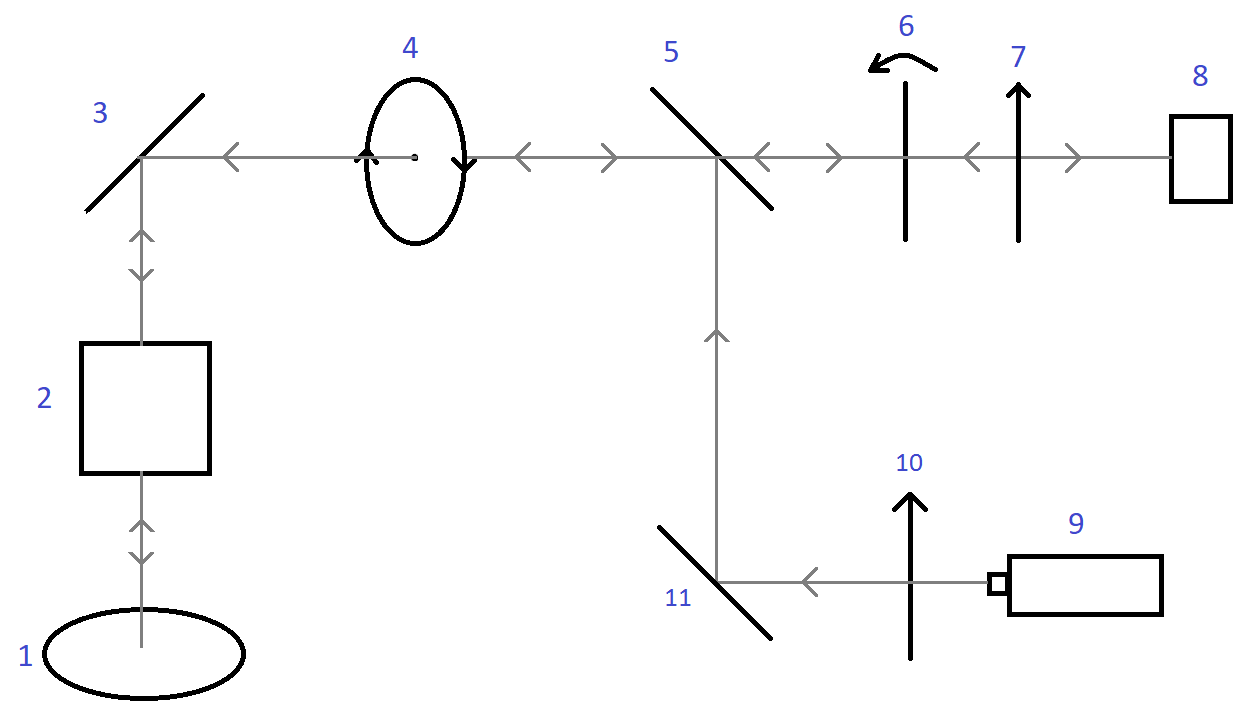
\includegraphics[width=1.0\linewidth]{Przygotowania/Uklad-pomiarowy.png}
		\caption{Schemat układu pomiarowego.}
	\end{center}
\end{figure}

\begin{itemize}
	\item 1 - badana próbka, $\alpha$-$\mathbf{Ga_{2}S_{3}}$;
	\item 2 - Mikroskop;
	\item 3, 11 - Lustra;
	\item 4 - HWP\footnote{HWP z angielskiego ''Half-wave plate'' czyli  płytka półfalowa}, nazwa skrócona ''półfalówka'';
	\item 5 - Płytka pólprzepuszczająca;
	\item 6 - HWP 90$^{\circ}$, ustawiona tak że przekręca polaryzację o 90$^{\circ}$;
	\item 7, 10 - Polaryzatory;
	\item 8 - Detektor;
	\item 9 - Laser argonowy 514 nm;
\end{itemize}

Promieniowanie elektromagnetyczne o długości fali 514 nm, emitowane laserem argonowym (9), przechodzi przez pionowo ustawiony polaryzator (10). Chociaż fala elektromagnetyczna emitowana laserem już jest spolaryzowana, polaryzator (10) zapewnia dodatkową polaryzację. Dalej fala elektromagnetyczna odbija się od zwierciadła (11) i trafia na płytkę półprzepuszczającą (5). Zatem odbija się od tej płytki i przechodzi przez HWP (4), gdzie polaryzacja skręcona o określony kąt $\alpha$, po przejściu przez (4) polaryzacja fali elektromagnetycznej jest przekręcona o kąt 2$\alpha$. Dalej fala trafia na próbkę (1) przez (2). Rozproszona fala elektromagnetyczna na fononach trafia na zwierciadło (3), odbija się od tego zwierciadła i przechodzi prze ''półfalówkę'' (4). Teraz ''półfalówka'' względem światła rozproszonego ma skręcony kąt o $-\alpha$. Po przejściu przez (4) polaryzacja rozproszona fala elektromagnetycznej jest skręcona o -2$\alpha$. Dalej światło rozproszone trafia do ''półfalówki'' na stale przekręconej o 45$^\circ$ czyli fala, która przeszła przez (6) ma skręcony kąt polaryzacji o 90$^\circ$. Następnie po przejściu polaryzatora (7) fala elektromagnetyczna trafia na detektor z kamerą CCD. Polaryzator (7) jest po to aby zbierać światło rozproszone tylko o określonej polaryzacji.

Pomiar się odbywał w dwóch konfiguracjach:
\begin{itemize}
	\item VV - zbierane światło rozproszone w takim samym kierunku jak światło pobudzające\footnote{Światło emitowane laserem}. Bez HWP 90$^{\circ}$.
	\item VH - zbierane światło rozproszone w kierunku prostopadłym do światła pobudzającego. Z obecnością HWP 90$^{\circ}$.
\end{itemize} 

Charakterystyki pomiaru:
\begin{itemize}
	\item 1
\end{itemize}

\textbf{Zdjęcie i opis sprzętu pomiarowego, razem z oprogramowaniem}.

Przy pomiarach powstawały niektóre trudności.

Płytka $\mathbf{GaP}$ ma wymiary 3mm x 2mm x 1mm. Płytki kryształki które zostały utworzone na tej płytce były rzędu kilku mikrometrów. Poszukiwany kryształek do badań powinien przypominać sześciokąt, być osobnym kryształkiem i mieć płaską powierzchnię. Ta powierzchnia powinna być w miarę równoległa do podłoża.

Kryształki zostały utworzone na podłożu z $\mathbf{GaP}$. Piki na widmie ramanowskim pochodzące z galu nakładają się na niektóre piki pochodzące z $\mathbf{Ga_{2}S_{3}}$. To bardzo utrudnia analizę niektórych pików z $\mathbf{Ga_{2}S_{3}}$.

Kryształki zostały zdrapane papierem ściernym i przełożone na taśmę klejącą. Ale po kilku pomiarach ciepło które pochodzie od tego że promieniowanie laserowe grzeje miejsce w które trafia. Taśma klejąca pod wpływem ciepła rozszerza się, co powoduje znaczącą rozkalibrację układu pomiarowego. 

Zostało podjęte ryzyko, że zdrapane kryształki należy przenieść na szklaną płytkę. Z tej płytki te kryształki można łatwo zdmuchnąć. To jest niebezpieczne dla tego, że cały pomiar może być robiony przez dwa dni po kilku godzin.

\textbf{Zdjęcie badanego kryształku}. 

\subsection{Technologia wzrostu kryształków}

Kryształki zostały przygotowane w (gdzie?) i dostarczone na Wydział Fizyki PW. 

Metoda LPCVD - jest chemiczną technologią osadzania z fazy gazowej, która wykorzystuje ciepło do inicjowania reakcji gazu prekursorowego na stałym podłożu. Ta reakcja na powierzchni jest tym, co tworzy materiał fazy stałej na podłożu. Niskie ciśnienie (LP) stosuje się w celu zmniejszenia niepożądanych reakcji w fazie gazowej, a także zwiększa jednolitość tworzonej fazy na podłożu.

$[Ga(SiPr)2(\mu-SiPr)]2$ może być stosowany do osadzania sześciennego Ga2S3 w 723 K. Po wyżażaniu laserowym tworzy się monoclinic.

Przemiana fazowa zachodzi pomiędzy 773 a 873 K. 

























 